\subsection{\href{http://www.seconsat.com}{Seconsat}}
   \hypertarget{subsec:seconsat}
   Ademas de las tareas de consultoría, se desarrolló un equipo inalámbrico para reporte de temperatura, humedad, velocidad, y demás parámetros desde la caja de un camión de carga a un equipo rastreador. \\
   Se utilizó tecnología 0402 en una placa de 4 capas con requerimientos de radiofrecuencia desde 200 Mhz hasta 2.4 Ghz. \\
   Se definieron los requerimientos, se diseñó el esquematico, y se diseñó el PCB en Orcad Allegro como se muestra en la figura \ref{fig:seconsat1}.
   \begin{figure}
      \begin{center}
         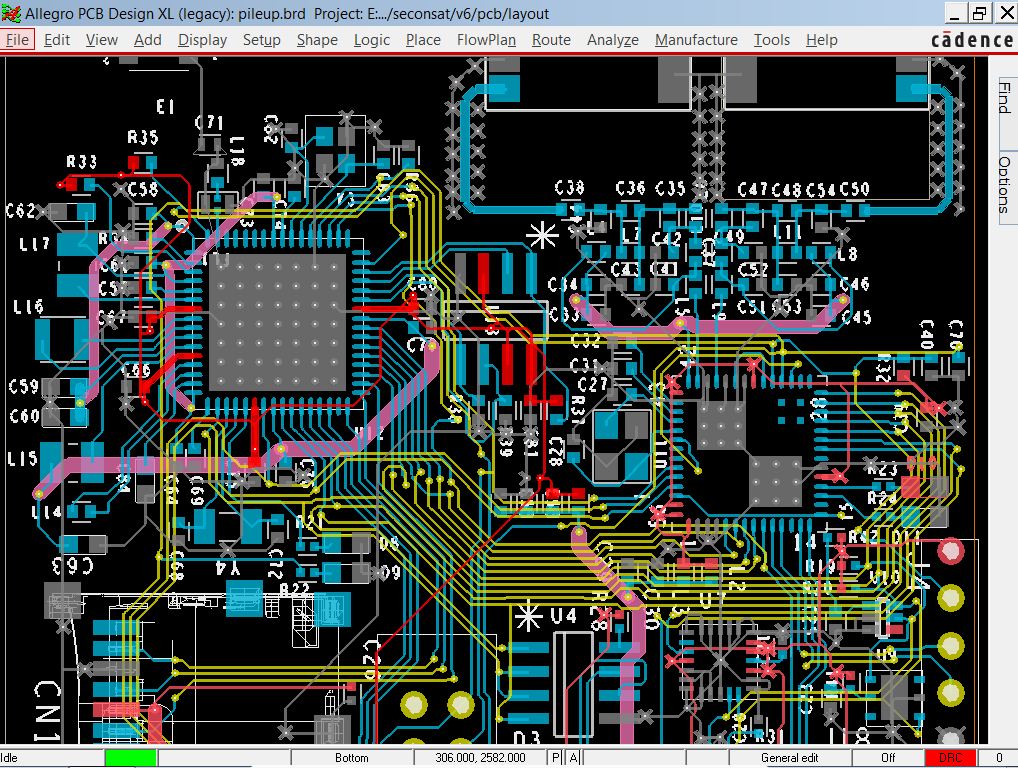
\includegraphics[width=0.49\textwidth]{./portfolio/seconsat1.png}
         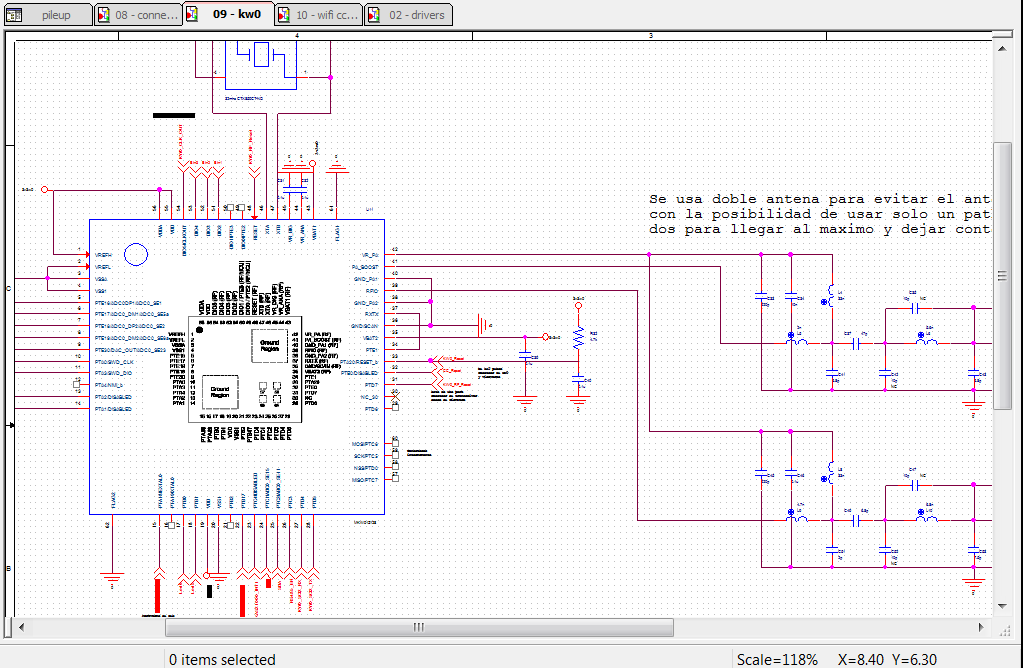
\includegraphics[width=0.49\textwidth]{./portfolio/seconsat2.png}
      \end{center}
      \caption{Desarrollo de PCB de comunicación inalámbrica 2.4Ghz y sub-1Ghz para reporte de parámetros ambientales dentro de camiones}
      \label{fig:seconsat1}
   \end{figure}

